\clearpage
\phantomsection

\setcounter{chapter}{1}
\chapter[{NHẬN DẠNG KÊNH TRUYỀN SỬ DỤNG THUẬT TOÁN BÁN MÙ MRE}]{Nhận dạng kênh truyền sử dụng thuật toán bán mù MRE}

\section{Sơ lược về thuật toán B-MRE}

Generally, MRE uses an $N$-taps linear equalizer to filter each channel. Let $g_{t, i}  \in \mathbb{C}^{LN \times 1}$ be an $i$-delay equalizer and $t$-th transmitter. For \mbox{$i=0, \ldots, K-1$}, at time $n$, we have
\begin{equation}
    g^H_{t, i} * x(n)=\sum_{l=0}^{L-1}\sum_{k=0}^{N-1} g^H_{t,i}(k) x^{(l)}(n-k) \approx s_t(n-i)
\end{equation}
% At $i$-delay, $g_i$ is express as follows
\begin{equation}
\begin{aligned}
    g_{t,i}=\big[g_{t, i}^{(0)}(0), \ldots, &g_{t, i}^{(0)}(N - 1), \ldots, \\
    &g_{t, i}^{(L-1)}(0), \ldots, g_{t, i}^{(L-1)} (N-1) \big]^\top
\end{aligned}
\end{equation}
The equalizers matrix for $t$-th transmitter is $G_t \in \mathbb{C}^{LN \times K}$ as follows
\begin{equation}
    G_t = [g_{t, 0}, \ldots, g_{t, K-1}]
\end{equation}

In the noise-free case, the transmitted symbols can be perfectly recovered with $\bar{G}$ is any left inverse of $\mathcal{H}$ since
\begin{equation}
    \begin{aligned}
        \relax[G_0, \ldots, G_{T-1}]^{H} 
        X(i)
        &= [S_0^\top(i), \ldots, S^\top_{T-1}(i)]^\top \\
        \bar{G}^H X(i) &= \bar{S}(i)
    \end{aligned}   
\end{equation}

In noisy case, to estimate $\bar{G}$, the MRE method exploits the delay diversity from multi-channel, $g_i^H X(i) = g_{i+1}^H X(i+1)$, to determine the full set of channel inverses. Where $g$ is the vector form of $\bar{G}$ equalizers matrix as shown in Eq.~\ref{eq:vecG} . The unconstrained MRE cost function of $\bar{G}$ is given by
\begin{equation}
    \mathcal{J}(\bar{G})=g^H \mathcal{R}g
\end{equation}
where $\mathcal{R} \in \mathbb{C}^{LNKT \times LNKT}$ is the matrix of $X(i)$ and $X(i+1)$ observed signals, which is given by
\begin{equation}
\label{eq:R}
\mathcal{R} \stackrel{\text { def }}{=} E\left(U^{H} U\right)
\end{equation}
with
\begin{equation}
\label{eq:U}
U = \left(I_{T (K-1)}, \mathbf{0}\right) \otimes X^{H}(i)-\left(\mathbf{0}, I_{T (K-1)}\right) \otimes X^{H}(i+1)
\end{equation}
Under the quadratic constraint~\cite{original}, the unique stable minimum of $g$ is estimated by selecting the smallest eigenvector of $\mathcal{R}$.


\section{Đề xuất phương pháp nhận dạng hệ thống SB-MRE cho MIMO}


In each transmitter, a block data $S_t$ is considered to send, including $N_p$ pilot symbols and $N_s - N_p$ data symbols.
\begin{equation}
S_t = \left[s(0), \ldots s\left(N_{p-1}\right), s\left(N_p\right), \ldots, s\left(N_s-1\right)\right]
\end{equation}

Pilot signals estimate the full set of channel inverse by the least-square method.
\begin{equation}
    \hat{G} = \arg \underset{\bar{G} \in \mathbb{C}^{LN \times KT}}{\min} \sum_{i=N-1}^{N_{p} - 1}\|\bar{S}(i)- \bar{G}^H X(i)\|_F^2 
\end{equation}

The combining of pilot-based and blind MRE is a constrained optimization that can readily solve by the Lagrange multiplier method~\cite{bertsekas2014constrained}. The total cost function of SB-MRE will be
\begin{equation}
\label{eq:cost}
    \mathcal{J}(\bar{G})=\sum_{i=N-1}^{N_{p} - 1}\|\bar{S}(i)- \bar{G}^H X(i)\|_F^2 +\lambda g^H \mathcal{R} g
\end{equation}
with $\lambda$ is a weighting factor, $\mathcal{R}$ in the quadratic form of the blind MRE criterion as shown in Eq.~\ref{eq:R}, and $g$ is the vector form of $\bar{G}$.
\begin{equation}
\label{eq:vecG}
    \begin{aligned}
        % g = \operatorname{vec}(\bar{G}) &=\left[\vec{G}_0^\top, \vec{G}_1^\top, \ldots, \vec{G}_{T-1}^\top\right]^\top \\
        % \vec{G_t} &= \left[\begin{array}{ll}
        % g_{t, 0}^\top, \cdots, g_{t, K-1}^\top
        % \end{array}\right]^\top
        g = \operatorname{vec}(\bar{G}) &=\left[\vec{G}_0^\top, \vec{G}_1^\top, \ldots, \vec{G}_{K-1}^\top\right]^\top \\
        \vec{G_i} &= \left[\begin{array}{ll}
        g_{0, i}^\top, g_{1, i}^\top, \cdots, g_{T-1, i}^\top
        \end{array}\right]^\top
    \end{aligned}
\end{equation}

Without loss of generality, the least-square expression of Eq.~\ref{eq:cost} is conjugate transposed and the sum operator is turned into matrix forms of $\widetilde{S}$ and $\widetilde{X}$. The cost function is expressed as follows
\begin{equation}
    \begin{aligned}
    \mathcal{J}(\bar{G})&=\sum_{i=N-1}^{N_{p} - 1}\left\|{\bar{S}(i)^H}-X(i)^H \bar{G}\right\|^2_F +\lambda g^H \mathcal{R} g\\
    &=\left\|\widetilde{S}^H-\widetilde{X}^H \bar{G}\right\|^2_F +\lambda g^H \mathcal{R} g
    \end{aligned}
\end{equation}
where $\widetilde{S}, \widetilde{X}$ are the matrices of shape $\mathbb{C}^{KT \times (N_p -N +1)}$ and $ \mathbb{C}^{LN \times (N_p-N+1)}$, respectively.
\begin{equation*}
    \begin{aligned}
        \widetilde{S} &= [\bar{S}(N-1), \ldots, \bar{S}\left(N_{p} - 1\right)] \\
        \widetilde{X} &= [X(N-1), \ldots, X\left(N_{p} - 1\right)]
    \end{aligned}
\end{equation*}

The least-square expression is vectorized and thanks to the property for vector, i.e., $\operatorname{vec}(AXB) = (B^\top \otimes A) * \operatorname{vec}(X)$. The SB-MRE cost function turned into
\begin{equation}
\label{eq:cost_final}
    \begin{aligned}
    \mathcal{J}(g) &= \left\|\operatorname{vec}(\widetilde{S}^H) - (I_{KT} \otimes \widetilde{X}^H) \operatorname{vec}(\bar{G})\right\|^2_F + \lambda g^H \mathcal{R} g\\
         &= \left\| \bar{s} - A g \right\|^2_F + \lambda g^H \mathcal{R} g \\
         &= g^H A^H A g + \left\| \bar{s} \right\|^2_F - 2\mathfrak{Re} (g^h A^H \bar{s}) + \lambda g^H \mathcal{R} g    \end{aligned}
\end{equation}

In order to find minimum cost of Eq.~\ref{eq:cost_final}, let derivative $\mathcal{J}(g)$ with respect to $g$ as follows
\begin{equation}
\begin{aligned}
\frac{\partial \mathcal{J}}{\partial g}(g) &= 0 \\
\left(A^H A+\lambda \mathcal{R}\right) g &= A^H \bar{s}
\end{aligned}
\end{equation}

The final equalizers matrix in vector form of the proposed SB-MRE method is obtained through
\begin{equation}
    g_{SB}=\left(A^H A + \lambda \mathcal{R}\right)^{-1} A^H \bar{s}
\end{equation}

\section{Đề xuất giảm thiểu chi phí của thuật toán SB-MRE}


In the ensuing, 

\subsection{Giảm thiểu độ phức tạp của thành phần B-MRE}
In the original work, the overall complexity of the blind MRE method is $\mathcal{O}(LNKT)$~\cite{original}. All $K$ equalizers are estimated for each transmitter, but only one is used in the final. This burden computation is not necessary when $N$ becomes bigger. Hence, in this section, we considerably reduce the number of equalizers to 2, i.e., the $0$-th and \mbox{$(K-1)$-th} equalizer. Now, the overall complexity is $\mathcal{O}(LNT)$ and equalizers matrix for $t$-th transmitter is given by
\begin{equation}
    V_{t} = [g_{t, 0}, g_{t, K-1}]
\end{equation}
Followed by the estimated signal source of $t$-th transmitter will be
\begin{equation}
    V_t^H X(i) = [s_t(i), s_t(i-K+1)]^\top = S_{t}(i)
\end{equation}
Following that, we do not have to compute the full rank of $\mathcal{R}$ as the blind approach. Eq.~\ref{eq:U} is modified to
\begin{equation*}
U = \left(I_{T}, \mathbf{0}\right) \otimes X^{H}(i)-\left(\mathbf{0}, I_{T}\right) \otimes X^{H}(i+K-1)
\end{equation*}
// Proof 
\subsection{Giảm thiểu độ dài chuỗi pilot}
In this section, we tried to find the minimum number of pilots ...

\section{Mô phỏng và đánh giá}

In this section, we illustrate the behavior of the proposed SB-MRE with the simulation parameters as shown in Table~\ref{tab:simulation_param}. The simulation results are averaged of 1000 running times. We first compare the performance of proposed SB-MRE versus traditional channel estimation algorithms, i.e., Zero Forcing (ZF) and Minimum mean square error (MMSE)~\cite{Jiang2011}, in terms of symbol error rate (SER). Fig.~\ref{fig:performance} shows that at lower SNR values, ZF and MMSE outperformance the proposed SB-MRE. Because the effect of B-MRE at lower SNR is negligible. However, the proposed SB-MRE hits the SER of ZF and MMSE at $\text{SNR}=7~\text{dB}$. Moreover, SB-MRE's SER is better than both traditional channel estimation methods at higher SNR. Note that the proposed SB-MRE in this simulation only uses $32/256$ symbols for pilots. On the other hand, ZF and MMSE require full acknowledgment of channel state information (CSI). After reducing the cost of B-MRE component, the performance of SB-MRE\_rc is still better than that of original B-MRE and B-MRE\_rc. With $\text{SNR values of~}19~\text{dB}$ and higher, SB-MRE\_rc finally hits the perfect SER.


\begin{table}[H]
\centering
\caption{Simulation parameters}
\label{tab:simulation_param}
    \begin{tabular}{p{6cm} | p{4cm}}
    \hline
    \hline
    \textbf{Parameters} & \textbf{Specifications}  \\ \hline
    MIMO                            & $T = 2, L= 4$      \\ \hline
     Modulation                     & QPSK       \\ \hline
    Channel order                   & $M = 3$      \\ \hline
    Windows size                    & $N = 10$     \\ \hline
    Sample size                     & $N_s = 256$  \\ \hline
    Pilots                          & $N_p = 32$   \\ \hline
    Number of blind equalizers      & $2$ \\ \hline
    Weighting factor                & $\lambda = 0.1$   \\ \hline
    \end{tabular}
\end{table}


\begin{figure}[ht]
    \centering
    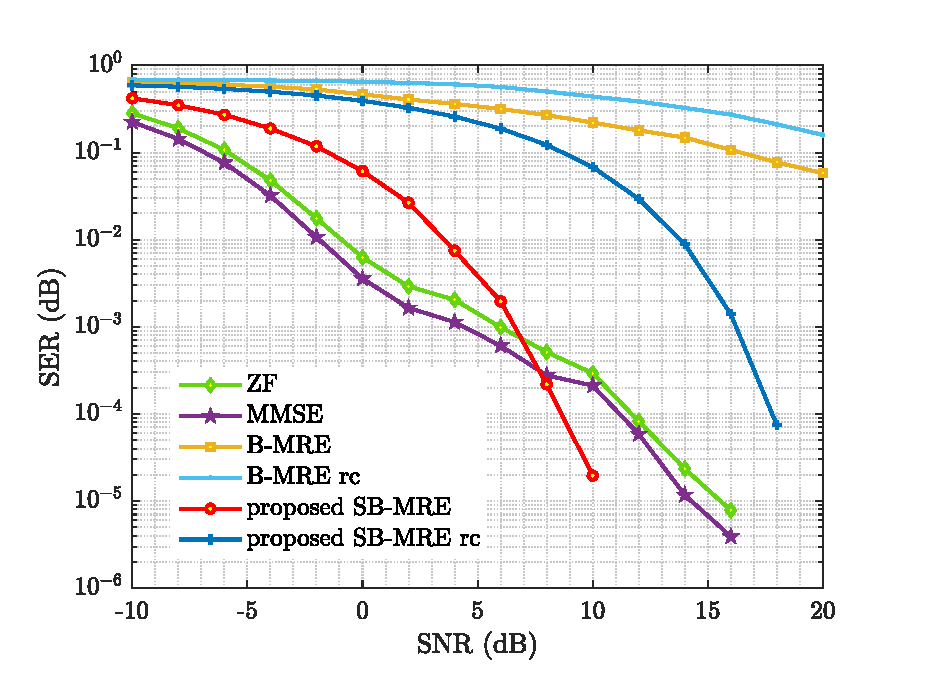
\includegraphics[width=.8\linewidth]{figures/performance.eps}
    \caption{Proposed SB-MRE for channel estimation.}
    \label{fig:performance}
\end{figure}

After that, we simulate to verify the performance of proposed SB-MRE in different numbers of pilots ($N_p$) and SNR values. As shown in Fig.~\ref{fig:vary_N_p}, $N_p$ and SNR are turned in range $[10 \;\; 64]$ pilot symbols and $[5, 10, 15]$~dB, respectively. Overall, the SER curves of SB-MRE and SB-MRE\_rc gradually decrease when $N_p$ and SNR are larger. The behavior is the trade-off between spectrum efficiency and the accuracy of channel estimation algorithm. At $\text{SNR}=15~\text{dB}$, SB-MRE with $N_p > 30$ archives to perfect SER. For SB-MRE\_rc, when $N_p$ increases in range $[10 \;\; 20]$, SER curves clearly improve. But if $N_p > 20$, the SER curves almost keep stable. 
\begin{figure}[ht]
    \centering
    \begin{subfigure}
         \centering
         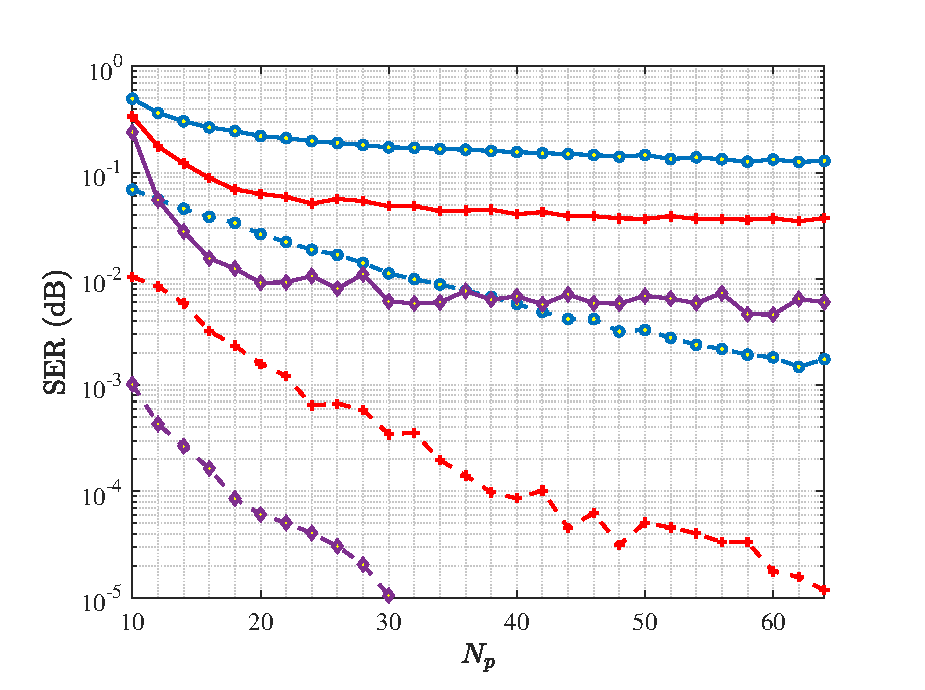
\includegraphics[width=0.8\linewidth]{figures/vary_N_p_1.eps}
     \end{subfigure}
     \hfill
     \begin{subfigure}
         \centering
         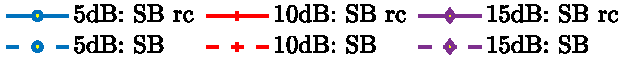
\includegraphics[width=.6\linewidth]{figures/legend.pdf}
     \end{subfigure}
     \hfill
    \caption{Performance of proposed SB-MRE with differs $N_p$ and SNR.}
    \label{fig:vary_N_p}
\end{figure}

Finally, we consider the effect of weighting factor ($\lambda$) between pilot-based and B-MRE. The $\lambda$ is turned in range $[0.01 \;\; 0.2]$. As illustrated in Fig.~\ref{fig:vary_lambda}, at lower SNR, i.e., $5, 10$~dB, the SER curves slightly reduce as $\lambda$ increases. However, $\text{SNR}=15~\text{dB}$, the B-MRE component's performance becomes significant, leading to the SER curve of SB-MRE\_rc markedly decreasing. At the same SNR level, the proposed SB-MRE gets perfect accuracy, as shown in Fig.~\ref{fig:performance}.

\begin{figure}
    \centering
    \begin{subfigure}
         \centering
         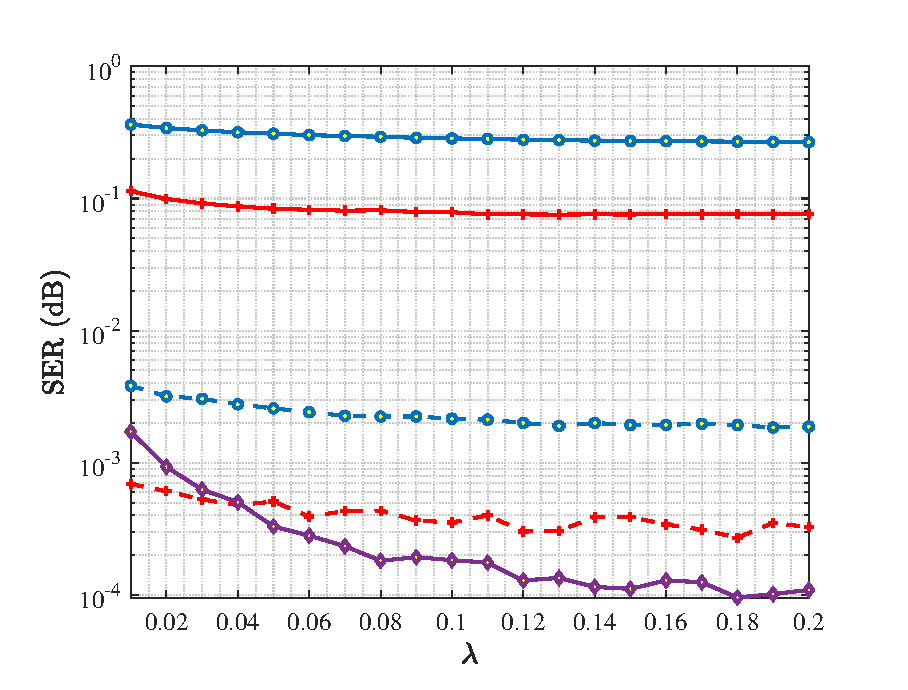
\includegraphics[width=.8\linewidth]{figures/vary_lambda.eps}
     \end{subfigure}
     \hfill
     \begin{subfigure}
         \centering
         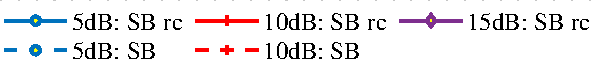
\includegraphics[width=.6\linewidth]{figures/legend_1.pdf}
     \end{subfigure}
     \hfill
    \caption{Performance of proposed SB-MRE with differs $\lambda$ and SNR.}
    \label{fig:vary_lambda}
\end{figure}